%
%  $Author: awl8049 $
%  $Date: 2009/06/06 19:30:19 $
%  $Revision: 1.1 $
%
%\documentclass[times,10pt,twocolumn]{article}
\documentclass[times,12pt,onecolumn]{article}
\usepackage{latex8}
\usepackage{setspace}
\usepackage{times}
\usepackage{graphicx}
\usepackage{authblk}
\usepackage{amsmath}
\usepackage{amsthm}
\usepackage{algpseudocode}
\pagestyle{empty}
\begin{document}
\title{Thermal Load Balancing of Server Workload Given Prediction of
  Thread Energy Consumption}
\author[]{Adam Lewis} 
\author[]{Soumik Ghosh} 
\author[]{N.-F. Tzeng}
\affil[]{Center for Advanced Computer Studies,University of Louisiana, Lafayette, Louisiana 70504\\ 
  \{awlewis,sxg5317,tzeng\}@cacs.louisiana.edu
}
\maketitle
\newtheorem{defn}{Definition}
\newtheorem{thm}{Theorem}
\thispagestyle{empty}
\doublespacing
\begin{abstract}

\end{abstract}

\section{Introduction}
\label{sec:Introduction}
Power management techniques developed for mobile and desktop computers
are not always appropriate for real-time and high-performance computing
applications as these techniques take advantage of slack periods that
occur within the application workloads. Real-time applications have
strict deadline requirements that cannot be impact by slowing down the
processor as required by DVFS. In the case of high-performance
computing, typical workloads result in the application server being
fully utilized with few resources available for reactive scheduling. As
such it becomes necessary to find power management techniques that are
pro-active in nature rather than reactive.

In this work, we introduce a technique for thermal
managagement that minimizes server energy consumption by adjusting the
allocation of thread groups to available cores so as to produce the
least contention for memory accesses amongst thread groups.   This must
be balanced against the performance benefits that are gained through
cache affintiy; by allocating thread groups to last utilzied cores as as
to gain performance by taking advantage of data still existing in cache
will lead to thermal issues through more active cache access.

\section{Prior Work}
\label{sec:prior}
\begin{verbatim}
Outline of pending changes:
* Need to add review of prior work in thermal load balancing.
* Current text is only reporting prior work, needs to be more critical
\end{verbatim}
Previous attempts to implement effective thermal management in
processors have taken two distinct approaches: hardware based
implementations of Dynamic Thermal Management (DTM) combined with Dynamic
Voltage-Frequency Sacaling (DVFS) or operating system based
multiprocessor or multi-core thread migration approaches.

Commercial processors crudely regulate thermal stress using DTM by
slowing down the processor using DVFS whenever processor temperature
exceeds a certain threshold.  A categorization of the different thermal
management techniques based on this approach can be found in
\cite{Donald2006}.  In this work, the authors claimed the best approach
to using DTM/DVFS includes a combination of a control-theoretic
distributed DVFS system and a sensor-based migration policy.  The issue
with this approach is the granularity of DVFS; existing commercial
systems do not allow for independent frequency scaling of cores and
threads.

The idea of migration of work for energy savings and thermal management
has a long history in the SMP, SMT, and CMP environments
\cite{Yao1995}. Static methods been applied in attempts to solve this
problem.  In \cite{Coskun2008}, integer linear programming was used to
obtain a task schedule that met real-time deadlines while attempting to
minimize hotspots and spatial temperature differentials across the die.

Examples of dynamic methods to solve this problem incude Heat-and-Run
\cite{Gomaa2004},HybDTM \cite{Kumar2006}, and ThreshHot \cite{Yang2008}.
Heat-and-Run proposed to distribute work amongst available cores until
the DTM events occur and then migrate threads from the overheated cores
to other non-heated coraes. HybDTM combined DTM techniques with a thread
migration strategy that reduces the thread priority of jobs on cores
that are running hot. ThreshHot uses an on-line temperature estimator to
determine in what order threads should be scheduled onto cores. In all
three cases, these techniques utilize data from hardware performance
counters and hardware temperature sensors to guide the scheduling
decision.

A related approach to migration is to control the CPU time slice
allocation.  In \cite{Bellosa2003}, it was proposed to modify the
process scheduler to allocate time slices as indicated by the
contribution of each task to the system power consumption and the
current temperature of the processor. A variation on this scheme was
proposed in \cite{Li2008} where system level compiler support was used
to insert run-time profiling code into applications to provide hints to
the thermal intensity of a task. In \cite{Merkel2008}, a scheduling
policy was proposed that sorts the tasks in each core's run queue by
memory intensity so as to schedule memory-bound tasks at slower
frequencies.

\subsection{Power and Energy Models}
\label{sec:models}
Power models are used to predict to when to apply power management
techniques to a working system. These models can be classified into two
broad categories: detailed analytical power models and high-level
blackbox models~\cite{Rivoire2008b}. Analytical models use detailed
knowledge of the underlying hardware to either simulate the energy
consumption or directly measure energy comsumption at the hardware
level.  Simulation can provide detailed analysis and breakdown of energy
consumption; however, they are slow and do not scale well to realistic
applications and large data sets.  Simulation-based models do not fit
well into scensarios where dynamic optimization of application
performance is required~\cite{Economou2006}. 

High level black-box models sacrifice some accuracy by avoiding
extensive detailed knowledge of the underlying hardware.  At the
processor level, \cite{Contreras2005}, and \cite{Bellosa2003} created
power models that linearly correlated power consumption with performance
counters. Models have been built for the processor, storage devices,
single systems, and groups of systems in data centers.  These models
have the advantage of being simple, fast and low-overhead but do not
model the full-system power consumption.

Measurement-based models attempt to collate power measurements with
hardware and software performance metrics.  Two distinct classes of
metrics have been used in these models: processor performance counters
and operating system performance metrics.  Processor performance
counters are hardware registers that can be configured to count various
microarchitectural events such as branch mispredictions and cache
misses.  In general, the number of countable events exceed the number of
available registers.  As result, models that use these counters
time-multiplex different sets of events on the available registers.
While this allows for more events to be monitored, it results in
increased overhead and lower accuracy due to sampling
issues~\cite{Economou2006}\cite{Rivoire2008a}.

Attempts have been made to reconcile these approaches by attempting to
map programs phases to events \cite{Isci2006}.  The most common
technique used to associate PeCs and/or operating systems metrics to
energy consumption use linear regression models to the collected metrics
to the energy consumed during the execution of a program
\cite{Contreras2005}\cite{Economou2006}\cite{Isci2003b}\cite{Bircher2007}.

In server envrionments, it has been shown that full-system models
using operating system CPU utiliziation can be highly
accurate~\cite{Fan2007}. Others have used similar
approaches~\cite{Heath2005} to develop linear models for energy-aware
server consolidation in clusters.  Full-system models such as
MANTIS~\cite{Economou2006}\cite{Rivoire2008a} relate usage information
to the power of the entire system rather than an individual component.
The accuracy and portability of full system power models is considered
in~\cite{Rivoire2008b}.  This analysis indicated that to ensure
reasonable accuracy across machines and workload required a model based
on a combination of both PeCs and operating system metrics.
\section{Background}
\label{sec:background}
It is the role of the kernel dispatcher to manage the placement of
threads in a dispatch queue, decide which thread to run on a processor,
and manage the movement of threads to and from processors.   At the
fundamental level, the kernel dispatcher is a queue management system
that must perform four core functions~\cite{McDougall2007}: (1) queue
management, (2) thread selection, (3) processor selection, and (4)
context switching.
\subsection{Solaris Power-Aware Dispatcher}
\label{sec:solpad}
OpenSolaris defines locality groups (lgroups) to provide a
locality-oriented mechanism to represent a collection of CPUs and
memory resources that are within some latency of each other.
Lgroups are hierarchical and are created automatically by Solaris
based on the system’s configuration and different levels of
locality. The system places a new thread into a home lgroup that
is based on load averages although applications can give a thread
a different home lgroup. Lgroups help to control where threads
and memory are allocated.  When a thread is scheduled to run, the
thread is assigned to the available CPU nearest to the home
lgroup, and memory is gotten either from the home lgroup or some
parent lgroup.

Inside the Solaris kernel, logical CPUs will belong to one or more CPU
partitions.  An overall system CPU partition is created at system
initialization.  At the user level, a logical CPU will be a member of
one or more processor groups.  Processor groups are implemented inside
the kernel as CPU partitions.
\begin{figure}
  \centering
  \includegraphics[scale=0.40]{padarch.pdf}k
  \caption{Solaris Power-Aware Dispatcher design.}
  \label{fig:padarch}
\end{figure}
The Solaris Power-Aware Dispatcher (PAD) (Figure~\ref{fig:padarch})
\cite{Sun2009} extended the Solaris kernel dispatcher to enumerate
logical CPUs that represent active and idle power domains.  The concept
of processor groups has been extended to include the concept of logical
CPUs sharing one of two power domains: active and idle.  At system
start-up, the dispatcher will query the operating system's power manager
to determine if a logical CPU is a member of either of these domains.
If so, the CPU is added to the appropriate processor group.  As the
workload progresses, the power manager tracks utilization in each power
domain.  The power manager utilizes this information to decide how to
change power states for each CPU.  This capability allows the dispatcher
to attempt to concentrate light workloads on a smaller number of logical
CPUs and make more resources available for scheduling.

\subsection{Energy Models and Performance Counters}
\label{sec:energymodels}
The foundation of our scheduler is the model for run-time energy
consumption detailed in \cite{Lewis2008}. This model provides a
system-wide view of the energy consumption by using hardware performance
counters to relate system power consmption to its overall thermal
envelope.

Modern processor cores support between 30 to 500 PeCs (depending upon
the processor) but only permit 2 to 18 of these counters to be read at
one time (again depending upon processor).  Furthermore, certain
combinations of PeCs may not be permitted to be collected at the same
time. Using PeCs to gain insight into architectural events (in our case
bus transactions)is complicated by the fact that the types of events,
number of events, and use cases varies widely, not only across
architectures, but across systems sharing the same Instruction Set
Architecture (ISA).  For instance, the Intel and AMD implementations of
performance counters have very little in common in spite of the
processor families using the same ISA~\cite{Singhal2008}\cite{AMD2008}.

As an example, to derive the thermal impact of application on cache, the
scheduler needs to collect nine PeCs to calculate shared and unshared
cache activity on the AMD Opteron processor: $RetiredInstructions$,
$DCAccesses$, $DCRefillsL2$, $DCRefillsFromSystem$, $ICFetches$,
$ICrefillsFromL2$, $ICRefillsFromSystem$, $L2RequestsTLB$, and
$L2MissesTLB$.  The model must calculate the L2 miss rate and L2 miss
ratio using the following set of formulas with the PeCs as inputs:
\begin{align}
  L2MissRate &= L2misses / RetiredInstructions\nonumber\\
  L2MissRatio & = L2misses / L2Requests\nonumber
\end{align}
These measures indicate cache activity which our model uses as an estimator
for energy consumption and potential for a DTM event.

Note that we have to collect nine different PeCs even though the
processor can only collect four of these counters at a time.  For
real-time situations, time multiplexing is the most popular solution to
this problem~\cite{Azimi2005}. In this approach the performance
counters are reconfigured for different sets of counter events at
regular time intervals.  However, time multiplexing introduces issues
with reconfiguration overhead and time alignment of samples.
\section{Thermal Model}
\label{sec:thermal}
\begin{verbatim}
Model is incomplete, needs additional discussion on meaning of terms
\end{verbatim}
There are two major metrics of interest for the thermal workload of a
multicore processor. The first is the total time of execution ( denoted
by $L$ for length ) of a certain application (denoted by $A$),

\begin{equation}
L(A(p_i),D_A,t)\nonumber
\end{equation}

where application $A$ has $p$ processes, each associated with a data set
of size $d_i$ in a single chip. $D_A$ is the total data associated with
application $A$, and $D_A = \sum_{i=1}^p{d_i}$.  We assume that the
activities are taking place in a staging area which contains the main
and virtual memory operating spaces, as well as the processor with its
cores and their associated caches and shared cache.

This time of execution measurement includes both computation time, and
the time to move the data for the problem from the staging area
(peripherals off the chip like DRAM and HDD) to a computation or
operation area (on the chip such as the caches and the cores).

The second major metric of interest is the energy consumption or energy
workload of an application, $U(A(p_i),d_i)$. For each application $A$
and problem size $D_A$, a measure of the workload, $W(A(p_i),d_i)$, is
defined in a data-operation dependent and system-independent way. W
contains two components, one being the operations count that is
performed by the computational core, and the other is the communication
operations in transferring data and instructions and data coherency and
book-keeping operations. These are measured in terms of the number of
bytes operated ON, or number of bytes transferred. Thus the energy
workload of an application $A$ operating on a data set $D_A$ can be
expressed as :

\begin{equation}
U(A(p_i),d_i) = \displaystyle \lim_{n \to k_e }n \times W(A(p_i),d_i) \times L_n(A(p_i),d_i,t) \nonumber
\end{equation}

where $L_n(k, d_i)$ is the total time to execute $n$ applications using
the chip. The term $k_e$ is the total number of applications that can be
excuted with the associated length of time for $L_n$, at which point a
``thermal event'' will occur causing the applications and the system to
catastrophically fail, or shut down.

It is easy to see that the above term is energy consumption of the
system till a thermal event occurs. In order to relate the energy
expenditure of the system while running applications, to teh
corresponding joule heating, we define the term ``Thermal equivalent of
Application'' (TEA), which is defined as the electrical work converted
to heat in running an application and is measured in terms of die
tmperature change and ambient temperature change of the system. Thus for
the application $A$ we express TEA as :

\begin{align}
\Theta_A(A(p_i),d_i, T, t) &= \frac{U(A(p_i),d_i)}{\displaystyle \lim_{T \to T_{th}} J_e \times (T - T_{nominal})}  \nonumber\\
					      &= \frac{\displaystyle \lim_{n \to k_e }n \times W(A(p_i),d_i) \times L_n(A(p_i),d_i,t)}{\displaystyle \lim_{T \to T_{th}} J_e \times (T - T_{nominal})} \nonumber
\end{align}

In these expressions, $T_{th}$ refers to the threshold temperature at
which a DTM triggered event will occur.  $T_{nominal}$ refers to the
nominal temperature as reported by the DTM counters / registers , when
only the operating system in operating and no application is being run.
The term $J_e$ is the ``electrical equivalent of heat'' for the chip,
which reflects the \textit{informational entropy} of the system
associated with processing the bits application $A(p_i)$ computes and
communicates, as well as the black body thermal properties of the chip
packaging and the cooling mechanisms around the chip. TEA thus is a
dimensionless quantity , both denominator and numerator being expressing
of work done or energy consumed in finishing a task.

For managing the thermal envelope of applications on server systems as
well as embedded systems, we are interested in the thermal efficiency of
the operation, that is, the thermal cost of taking an application to
completion. In general the efficiency $\eta(A(p_i), d_i,T)$ is defined
as

\begin{equation}
\eta(A(p_i), d_i,T, t) = \frac{\Theta_A(A(p_i),d_i, T, t)}{\Theta_A(A_e(p_i),d_i, T_{me}, t_e)} \nonumber
\end{equation}

where $T_(me)$ is the maximum temperature till which the core will carry
over till a DTM triggered event occurs. $A_e$ refers to the application
whose energy consumption has caused the DTM triggered event to take
place. $T_e$ is the execution time of application $A_e$. Thus
$\eta(A(p_i), d_i,T)$ is a measure of the ``thermal efficiency of the
application'', which implies how much an application affects temperature
change without compromising it's throughput and/or leads to a thermal
event. Thus the definition of $\eta$ is linked to the definition of the
thermal and energy workload.

An important metric finally is the achieved performance per unit power
consumed by the chip,
\begin{align}
C_{\theta}(A(p_i), d_i, T, t) &= \frac{\Theta_A(A(p_i),d_i, T, t)}{P(A(p_i),d_i)} \nonumber\\
	             			 &= \frac{\Theta_A(A(p_i),d_i, T, t)}{\displaystyle \sum^{chip,DRAM,HT,HDD} \int_{t=0}^{t=L_A}v(t)i(t)dt} \nonumber
\end{align}
where $P(A(p_i),d_i)$ is the overall power consumed during the
application lifetime. the quantity $\int_{t=0}^{t=L_A}v(t)i(t)dt$ is the
total power consumed by a single physical component (processor, DRAM
units, HDD, HT or FSB) during the length of the application $L_A$, with
$v(t)$ and $i(t)$ being the instantaneous voltage and currents
respectively.

This normalized quantity $C_\theta$ gives some indication of the
``cost'' of executing the benchmark on the given chip.

The final optimization function could be thought of as :
\begin{equation}
\frac{\partial^2 C_{\theta}(A(p_i), d_i, T, t)}{\partial T \partial t} = \frac{\partial^2}{\partial T \partial t} \frac{\displaystyle \lim_{n \to k_e }n \times W(A(p_i),d_i) \times L_n(A(p_i),d_i,t)}{\displaystyle \lim_{T \to T_{th}} J_e \times (T - T_{nominal})} \\
											       \times \frac{1}{\displaystyle \sum^{chip,DRAM,HT,HDD} \int_{t=0}^{t=L_A}v(t)i(t)dt} \nonumber
\end{equation}

\begin{verbatim}
Need to work mapping of model to physical quantities measured (PeCs,
other metrics)

This will be a table plus additional formulas
\end{verbatim}

\begin{figure}[htbp]
  \centering
  \includegraphics[scale=0.40]{schedarch.pdf}
  \caption{PAD thermal enhancement.}
  \label{fig:schdarch}
\end{figure}
\section{Design and Implementation}
\label{sec:design}
The design intent is for our scheduler to be
implemented as an extension to the existing dispatcher and power
management infrastructure in the operating system.  Our initial
prototype is an enhancement to the PAD as illustrated in
Figure~\ref{fig:schdarch}.
\begin{figure}[htbp]
  \centering
  \includegraphics[scale=0.40]{procgroup.pdf}
  \caption{Thermal processor groups.}
  \label{fig:thpg}
\end{figure}
\subsection{Extending Processor Groups for Thermal Management}
\label{sec:thenhance}
The concept of processor group is extended to include three new
processor domains organized by the temperature of the logical CPUs in
this time period: hot (90\% of DTM temperature), warm (between 75\% and
90\% of DTM temperature), and cold (less than 75\% of the DTM
temperature).  As the temperature of a logical CPU
increases, the processor core may be assigned to a different domain based on
how close the temperature is to causing a DTM event.  
\begin{figure}[htbp]
  \centering
  \includegraphics[scale=0.40]{thermalpredictor.pdf}
  \caption{Thermal predictor inputs.}
  \label{fig:predictor}
\end{figure}
The movement of logical CPUs between processor groups as temperature
increases is managed by a Thermal Predictor.  The Thermal Predictor
collects the values of the PeCs, temperature readings from the logical
CPUS, and utilization data from the dispatcher to decide whether a
processor will move towards the DTM temperature.  In this way we can
anticipate the DTM event and prevent its occurance.
\begin{figure}[htbp]
  \centering
  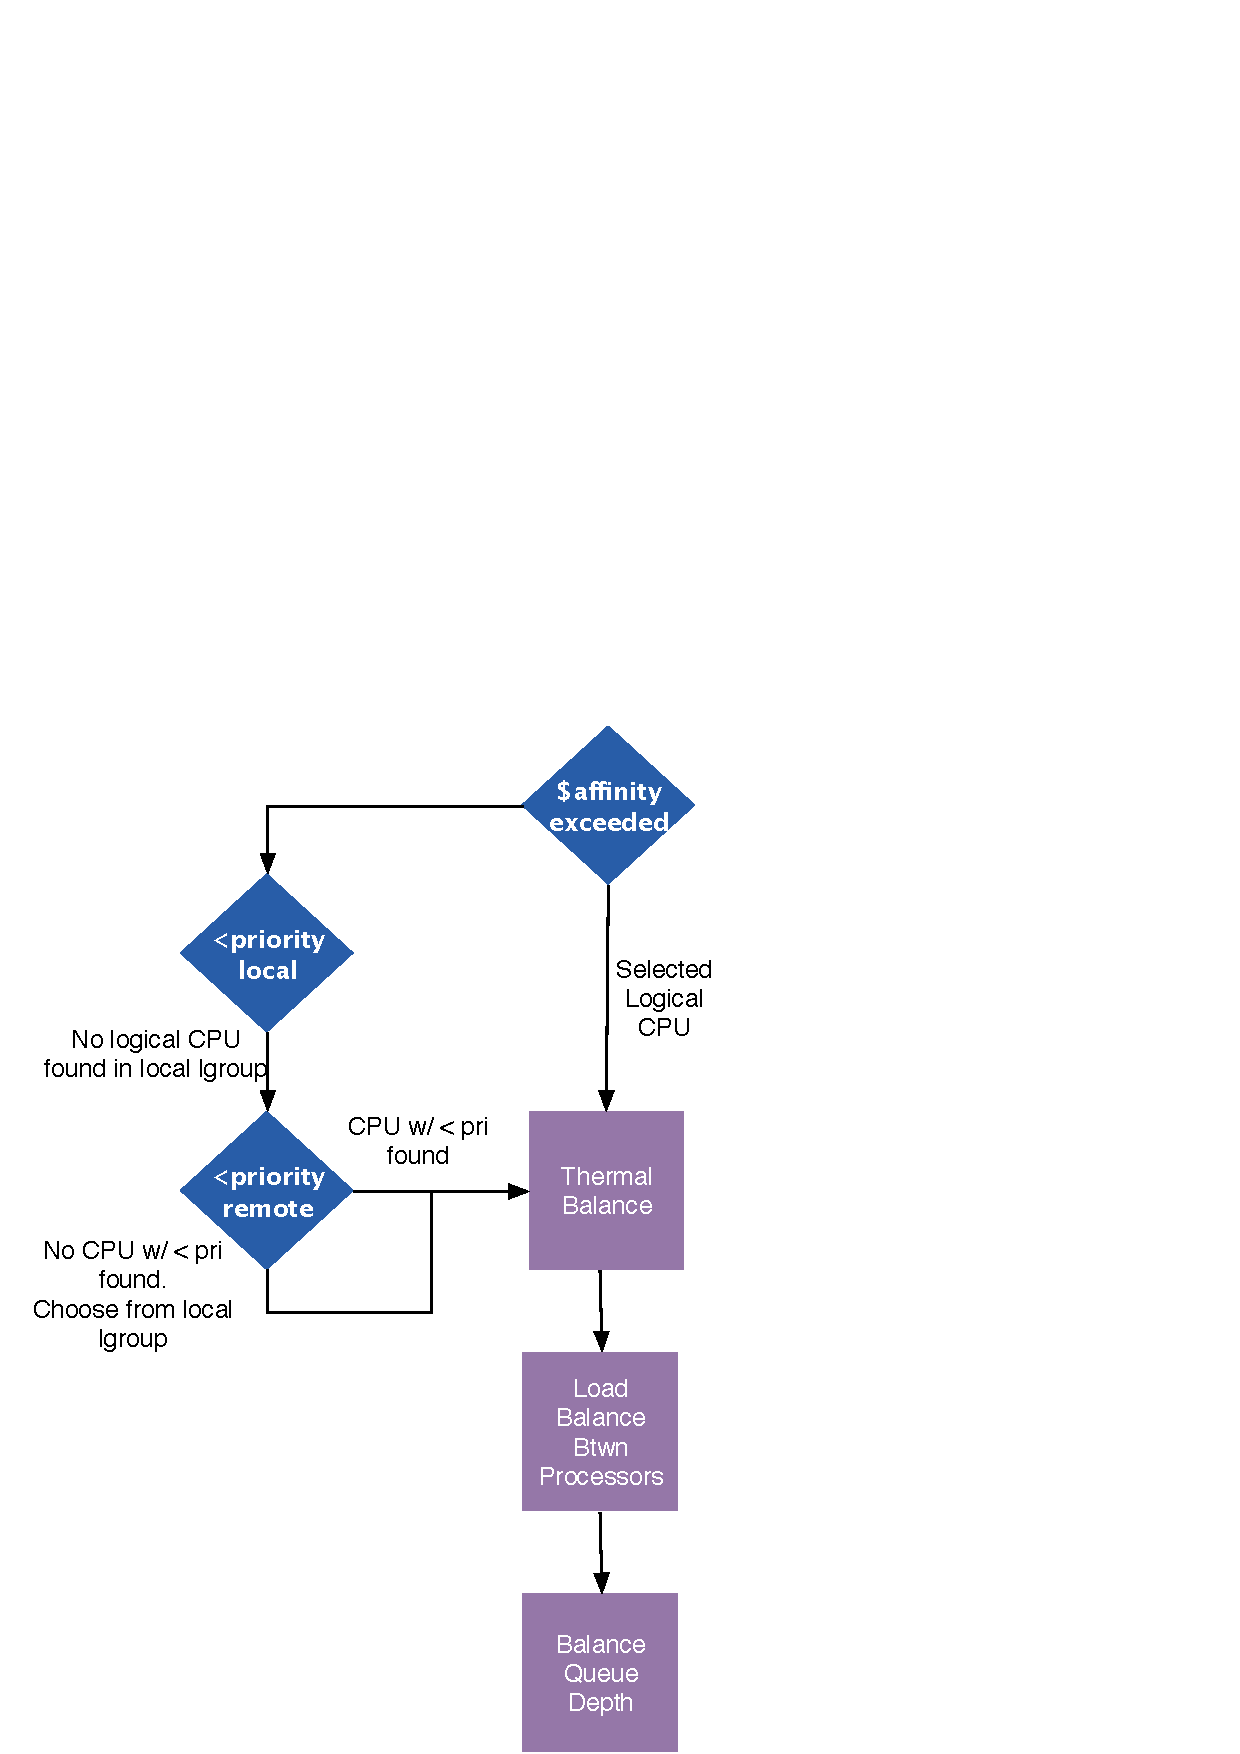
\includegraphics[scale=0.40]{threadinsert.pdf}
  \caption{Thread Queue Insertion}
  \label{fig:thread}
\end{figure}
The dispatcher is responsible for deciding where to insert threads into
run queues; i.e., when and where a thread will next execute. The steps
in this process are illustrated in Figure~\ref{fig:thread}.  First, the
dispatcher checks to see if the logical CPU where the thread was running
satisifies the cache affinity critieria (the default for OpenSolaris is
the thread was last running within the past 3 cycles).  If that test
fails, it tries to find the logical CPU in the local lgroup running the
lowest priority thread.  If no thread is found in the local lgroup, then
the dispatcher will check through known remote lgroups.  If no logical
CPU is found in either case, it will choose a logical CPU in the local
lgroup.

At this point, the system will attempt to load balance the workload.
Two possibilities exist in the current system: equal balance across all
physical processors in the system and coalese work onto one chip or the
other.  The first case is traditional example of load balancing while
the second case is attempting to free up as many resources as possible
to provide opportunities for power management to find logical units to
shut down.   We add a third sort of load balancing: temperature
balance. In this case, the dispatcher will attempt to load logical CPUs
in the ``COLD'' processor group first, followed by the ``WARM''
processor group, and finally the ``HOT'' group.


\section{Experimental Evaluation}
\label{sec:experiment}

\begin{verbatim}
Outline:
* Test required to validate thermal model issues
** Need to pin this down better with Soumik
* Compare four load balance policies:
** Existing OpenSolaris PAD coalese strategy (same as Heat&Run)
** Load balance scheme that models HybDTM
** Our HOT/WARM/COLD scheme
* Use two sets of benchmarks:SPEC2006 and SPECpower
\end{verbatim}

\section{Conclusions and Future Work}
\label{sec:conclusions}

\begin{verbatim}
TBD during period before submission
\end{verbatim}
\label{sec:references}
\small
\bibliographystyle{latex8}
\bibliography{hpca09.bib}

\end{document}

